\section{From Parametrized Surface Points to NURBS Representation}
As of yet, there is no open-source software which provides the conversion from a \textit{mesh-based} geometry to NURBS representation. Hence, one of the main challenges of both the algorithmic and implementation part of this project has been to develop one from scratch. Due to a variety of possible approaches to tackle this problem (e.g. \cite{ eck1996automatic, becker2011advanced}), we therefore conducted extensive prototyping work in MATLAB \cite{MATLAB} to avoid cumbersome and time-consuming implementation overheads during the prototyping phase. Once the algorithms to be used had been finalized, the prototypes were implemented a non-proprietary language, Python.

Following the example of using Peters' scheme to fit NURBS smoothly to datapoints in \cite{eck1996automatic}, we did extensive prototyping to ensure the tractability of using Peters' scheme (see \autoref{subsec:peters}) for fitting a NURBS surface (see \autoref{subsub:petersleastsq}) in our settings. As mentioned above, these prototypes were done in MATLAB, and were also partly implemented in Python. 

Incorporated in these algorithms were also the least-squares fitting with a Fairness Functional term (see \autoref{subsec:fairnessthry} and \autoref{subsec:lsqfairness}) to ensure surfaces without unnecessary sharp wiggles.

In the following part of this section, the implemented algorithm will be shortly described, based on the theory and notations in \autoref{sec:NURBS} and \autoref{sec:LSQfitting}.

\subsection{Algorithm}
The algorithm is given information about a quadrilateral mesh of vertices ($\petersControlMeshVec \in \petersControlMesh$), how they are connected into quads ($\verticesof{\hat{f}}, \forall \hat{f} \in \petersFaces$) as an ordered list of four vertex indices, and how they are parameterized (parameters $(u_\lsDataPoint, v_\lsDataPoint)$ and on which quad $\hat{f}\in\petersFaces$). The algorithm then roughly proceeds as follows:
\todourgent[author=erik]{{@}Saumi: can you homogenize this and next section and decide if both should have numerated lists or bullet points?}
\begin{itemize}
\item For every quad in the mesh, a $4 \times 4$ grid of points is created ($\petersPatchPoints$). In addition, lists are created of points with certain proximities to different corners of the quad, grouping together points from different quads with a similar relative position to a certain quad mesh vertex\footnote{These points are referred to with $A, B \text{and} C$ in \cite{peters1992constructing} and \cite{eck1996automatic}}.
\item For every datapoint $\lsDataPoint$ in the mesh, the parameters are first scaled from $\left[0,1\right]$ on the quad to $\left[0,1\right]$ on a local tensor product \Bez surface patch, related to the closest point in $\petersPatchPoints$. Then, the coefficients on the \Bez control points of this patch (corresponding to the datapoint's row in $\lsControlPointCoefMatrix(\vec{u}\vec{v})$) are calculated using the Bernstein polynomials, as described in \autoref{sec:NURBS}. 
\begin{itemize}
\item Then, the corresponding row in $\lsControlPointCoefMatrix(\vec{u}\vec{v})\lsControlPointCoefMatrix^{PS}$ is calculated, using a matrixless formulation of $\lsControlPointCoefMatrix^{PS}$. The matrixless formulation uses a combination of a precalculated table of coefficients for the points in Peter's scheme (calculated according to \cite{eck1996automatic}), together with with the lookup of point indices for points locations in $\petersPatchPoints$ created in the beginning of the algorithm. 
\item The row of $\lsControlPointCoefMatrix(\vec{u}\vec{v})\lsControlPointCoefMatrix^{PS}$ is saved in a sparse matrix\footnote{The sparse matrices for the surface reconstructed part are implemented using SciPy \cite{Numpy}}\todourgent[author=erik]{input the right citation of scipy}. 
\end{itemize}
\item For every point in $\petersPatchPoints$ (that is, for every \Bez patch), the precalculated coefficients of the Fairness functional (calculation described in \autoref{subsec:lsqfairness}) are applied to the \Bez control points of the patch to create one row of $\lsControlPointCoefMatrix^{fair}$. Using the same matrixless formulation as before, the corresponding row of $\lsControlPointCoefMatrix^{fair}\lsControlPointCoefMatrix^{PS}$ is calculated, and saved in another sparse matrix.
\item The fitting to datapoints and Fairness functional parts are combined by concatenating the datapoint matrix $\lsDataPointMatrix$ with a 3-dimensional $0$--vector, to form $\lsDataPointConcMatrix$, and by concatenating $\lsControlPointCoefMatrix(\vec{u}\vec{v})\lsControlPointCoefMatrix^{PS}$ and  $\lsControlPointCoefMatrix^{fair}\lsControlPointCoefMatrix^{PS}$ vertically to form $\lsControlCoefConcMatrix(\vec{u},\vec{v})$.
\item The mesh $\petersPatchPoints$ is calculated using sparse linear least squares\footnote{Also using SciPy.}.
\item The \Bez points of the patches are reconstructed from $\petersPatchPoints$, quad-wise, using a matrixless formulation of the second part of Peters' scheme, and the lookup of point locations calculated in the beginning of the algorithm.
\end{itemize}
At this point, we have reached the minimum we need for a reconstructed surface, now formulated as a network of tensor produduct \Bez curve surface patches of second and third order (quadratic and cubic). For conveniece, and usability, we convert them into one cubic tensor product NURBS curve surface patch per quad. That means the $4\times4$ \Bez patches per quad are turned into one cubic NURBS patch, with $13\times13$ control points. 
A sample result, the fitting of a surface to a toroidal shape defined implicitly for the \acs{DC} algorithm is shown in \autoref{fig:fittingStructures}. 
\begin{itemize}
\item First, the quadratic \Bez patches are degree-raised to cubic in both directions. \todointernal[author=erik]{add formula or reference to for example web page with a degree raising formula}. Then, since the cubic polynomial curves are shared between the patches along the edges, their four degrees of freedom, thus their control points, are shared along the edge.
\begin{itemize}
\item Then, we convert the \Bez patches into cubic B-spline or NURBS patches: the continous curves through the \Bez patch edges will have knots of triple multiplicity, with quadruple multiplicity along the edges of a quad to clamp the curve. \todointernal{Add any NURBS reference}
\end{itemize}
\item The NURBS patches are returned as a list of control points and an ordered array of indices for what control points belong to which quad.
\end{itemize}
%\item Implementations of the algorithm to calculate these \Bez point coefficients, as well as plotting them for debugging and visualisation
%\item \Bez curve and surface evaluation via calculating the coefficients on each \Bez control point from a set of parameters
%\item Algorithms to extract the necessary datapoints and parameters from the result data of the \acf{DC} algorithm in \autoref{ssec:DC}, using geometric conversions where necessary, and ignoring unusual datapoints
%\item An algorithm for using the four above algorithms to assemble the total coefficient matrix in \autoref{eqn:petersminimisation} in \autoref{subsub:petersleastsq}
%\item An application of MATLAB's built-in least squares minimisation tool to fit the resulting network of \Bez patches to the extracted surface.
%\end{itemize}


\begin{figure}
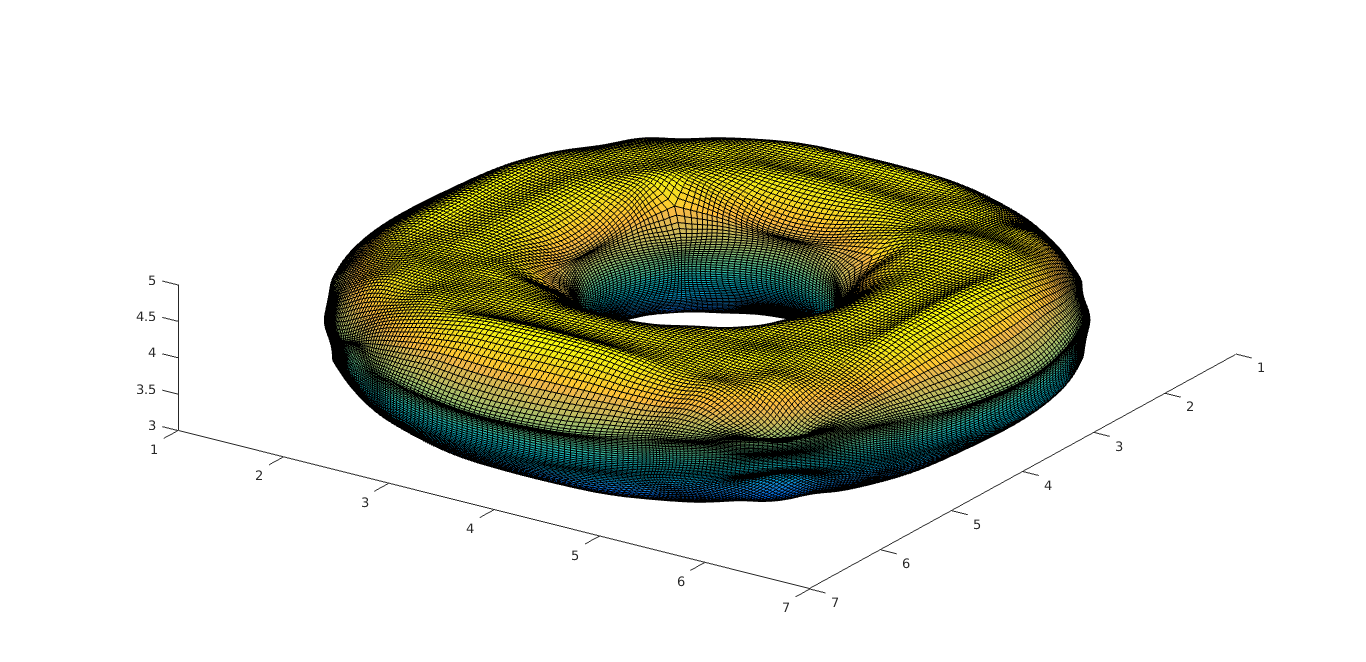
\includegraphics[width = \textwidth]{Pictures/NURBS/torus_from_DC.png}
\caption{A sample result from the Peters' scheme least-squares minimisation surface fitting, using the data provided by the \acs{DC} algorithm for an implicit function describing a torus. The grid lines on the figure are following the constant lines of each parameter value. As they follow the patch edges, corners where other than 4 coarse quads are meeting can be recognized, as for example on the middle of the far side of the torus, on the side that's facing the viewer.}
\label{fig:fittingStructures}
\end{figure}
\todourgent[inline,author=Benni]{From Bezier patches to NURBS using degree elevation. Add this to theory and implementation or only here?}


